\ifdefined\PROCINCLUDED
%
\else
%%% Please, do not change any of the following parameters.
\documentclass[b5paper,twoside,11pt]{article}
\usepackage[utf8]{inputenc}
\usepackage{geometry}
\voffset=-0.04cm
\headheight=0.6cm
\headsep=0.65cm
\textheight=19.5cm
\footskip=1.25cm
\voffset=-0.04cm
\textwidth=12.6cm
\marginparsep=0cm
\oddsidemargin=0cm
\evensidemargin=0cm
\marginparwidth=0cm
\usepackage{fancyhdr}
\usepackage{url}
\usepackage{graphicx}
\usepackage{mathptmx}
\usepackage{amsmath}
\usepackage{float}
\usepackage{subcaption}
\usepackage{placeins}
\usepackage{gensymb}
\usepackage{enumitem}
\usepackage{blindtext} 
\usepackage{tocloft}
\usepackage[labelsep=period]{caption}
\captionsetup[table]{skip=7pt}
\captionsetup[figure]{skip=6pt}
\fancyhead{}
\fancyfoot{}
\fancyfoot[LE]{\thepage}
\fancyfoot[RO]{\thepage}
\renewcommand{\headrulewidth}{0.4pt}
\renewcommand{\footrulewidth}{0pt}
\date{}
\def \papertitle#1{\title{#1}}
\pagestyle{fancy}
\def\insertauthor#1#2{
	\begin{minipage}[t]{.45\textwidth}
		\centering
		{\em#1} \\ \vspace*{0.25em}
		#2 \\ \vspace*{1.25em}
	\end{minipage}
}
\def\paperauthors#1{
	\author{
	\begin{minipage}[t]{\textwidth}
	\centering
	#1
	\end{minipage}
	}
}
\def\email#1{\\{\small\protect\url{#1}}}
\def\runningtitle#1{\fancyhead[CO]{\textit{#1}}}
\def\runningauthor#1{\fancyhead[CE]{\textit{#1}}}
\graphicspath{ {figures/} } %%% put all images file into "figures/" subdirectory

\begin{document}
\fi

\papertitle{Contribution title}
\paperauthors{
%%% insert one \insertauthor for each article author, \email part is optional
\insertauthor{Filip Rynkiewicz}{Lodz University of Technology \\ {\L}{\'o}d{\'z}, Poland\email{173186@edu.p.lodz.pl}}
\insertauthor{Stanis{\l}aw Nowak}{MacGilll University \\ Montreal, Canada}
}
\runningtitle{Contribution\dots} %%% brief title for running head
\runningauthor{Kowalski, J. et al.} %%% brief authors for running head


\graphicspath{ {images/} }


\maketitle




\begin{abstract}
Since the beginning of computer era we are trying to imitate nature. The results of those attempts are mathematical equations describing weather, snow flakes, plant growth or influence of species in individual biomes. In computer graphics fractal structure are often used because they can be simple characterize in mathematics. Those forms are common in nature. Self-similar fractals are created in computer graphics using Lindermayer Systems. This article was formed to analyse efficiency of this algorithm in modelling 3D tree triangle meshes for games. The general motivation of this topic is to produce way to procedural modelling and simplified edition of complicated 3D tree models. By combining L-systems with Bezier Curve there is a possibility to produce complicated 3D models. For example tree created with 468 branches having 87200 vertices and it is made in few seconds. In conclusion, time-consuming modelling in 3D programs can be replaced by solution described in this article. 
\end{abstract}

%%% insert your contribution here

\section{Introduction}
Using 3D modelling programs to create a complex 3D mesh of tree is very time consuming, because every branch has to be shaped separately.
To speed up and automatize this process Lindenmayer System can be used. Since 1968, when Aristid Lindenmayer created  grammatic to represent simple multicellular organism, technique has evolved. Now L-Systems are used to manage 3D models of plants\cite{Herbaceus}\cite{WebTree}\cite{Spray}\cite{wlosy}, fire visualization\cite{Sim}, music\cite{MLSystem} or even neural web\cite{LBrain}. Variaty os usage, flexibility and simplicity of this technique creates a possibility to extend it. Developers over years have used this technique to create software like L-studio\cite{L-Studio}, plugins to 3DsMax to animate plant growth\cite{ABartniak} or in Houdini\cite{LHoud}. Most of the algorithms to create 3D tree mesh are generating static models, to change or move branch user must change parameters inside L-System, and the recalculate the whole model. To prevent unnecessary actions and calculation the \textit{Bezier Curve} was added as the tree skeleton. Adding possibility of changing Bezier Points along Bezier Curve, user can change every branch only by moving it's handler and recalculating only this alternated branch.
\par After long years of plants observations the conclusion was brought, every plant can be treated as a very complex fractal. The most important feature of this structure is self-similarity. In mathematics, a self-similar object is exactly or approximately similar to a part of itself (i.e. the whole has the same shape as one or more of the parts)\cite{SelfSimi}. Because of complexity of plants as fractals the simplifications must be applied. To do this the L-System can be used.
Mentioned above technique is based on rewriting rules, so on replacing sub-terms of a formula with other terms. All formulas and terms are represented as strings, and L-system is all about changing one string to another based on rules. Every system has to have starting word, called axiom, rules of productions and number of iterations, so how many times rules must be applied to word. 

\section{Procedural Systems}

\subsection{DOL System}
Deterministic and context free L-system is one of the L-system, where context of the letter have no affect on algorithm. When axiom is \textit{b} and rules are: $b \rightarrow a$ and $a \rightarrow ab$ with 5 iterations, the example creation is shown at \figurename\ref{DOL}.

\begin{figure}[!htp]
\centering
  
\includegraphics[width=0.15\linewidth]{DOL-system}
\caption{Example of DOL system\cite{prusinABOP} \label{DOL}}
\end{figure}
\FloatBarrier
\subsection{Bracket L-System}
Using additional character in words user can create extra behaviors. L-system always create one long continued line. Using \textit{[} and \textit{]} the \textit{branches} can be created. First character is responsible for starting the branch and next for closing it. Branch is simply new line in geometric interpretation of string created by L-system.
\begin{figure}[!htp]
\centering
  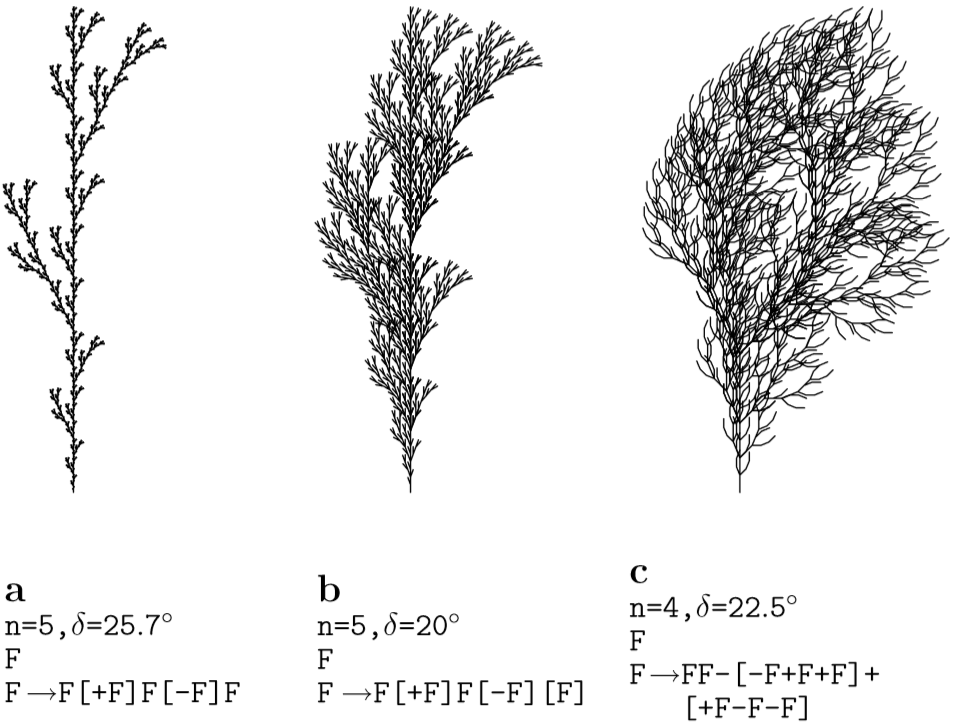
\includegraphics[width=0.7\linewidth]{branchingL}
\caption{Example of Bracket L-system\cite{prusinABOP} \label{branchingL}}
\end{figure}





\subsection{Parametric L-System}
To create more complicated models the Parametric L-System was created. Thanks to parameters L-system can change the values of variables, in example the steering angle of branch. When in DOL-System the sign \textit{+} was strictly assigned to hard-coded value, in this approach the value can be changed in every iteration using \textit{+(r)} where \textit{r} is some kind of parameter. Every letter or string must have brackets immediately behind it and within them there can be multiple parameters, separated with comma. Mathematical expressions can be applied between parameters.
\begin{equation*}
C(x\cdot e,e\backslash 2,a+c,b-d,g)
\end{equation*}
\subsection{Turtle interpretation of string}
L-System algorithm generates string, so it must be evaluated to create graphical content. Created word contains steering, drawing and omitted characters. The steering characters are the one which controls the behaviour of turtle. Drawn are those which simply adding a line between points.
\textit{Turtle graphics} is term where turtle have it's position, angle which describes the direction in which it is facing and any other parameters that user will use, but position and angle are mandatory.
Steering characters :
  \begin{itemize}  % local adjustment
\item[+] Turn  left  by  angle $\delta$.
\item[-] Turn right by angle  $\delta$.
\item[\&] Pitch down by angle  $\delta$.
\item[\string^] Pitch up by angle  $\delta$.
\item[\textbackslash] Roll left by angle  $\delta$.
\item[/] Roll right by angle  $\delta$.
\item[\string|] Turn around, by 180 $\degree $.
\item[[] Add branch.
\item[\char`\]] End branch.
\item[F] Draw line.
\end{itemize}	
Any Upper-case letter can be applied as a \textit{Draw line} command.
\section{Bezier Curves}
A B-spline is a generalization of the Bézier curve \cite{BSpline}. Let a vector known as the knot vector be defined 
\begin{equation*}
T={t_0,t_1,\ldots,t_m},
\end{equation*}
where \textbf{T} is a nondecreasing sequence with $t_i\in[0,1]$ and define control points \textbf{$P_0,P_1,\ldots,P_n$}. Define the degree as
\begin{equation*}
p\equiv m-n-1
\end{equation*}
The "knots" $t_{p+1},\ldots,t_{m-p-1}$ are called internal knots.


\begin{equation*} N_{i}^{j}(t)\;
\begin{cases} 1\qquad \;if \, t_i\leq t< t_{i+1}\:and\: t_i<t_{i+1} \\ 
0 \qquad   N_{i}^{j}(t)=\frac{t-t_i}{t_{i+j}-t_i} N_{i}^{j-1}(t) + \frac{t_{i+j+1} - t}{t_{i+j+1} - t_{i+1}} N_{i+1}^{n-1}(t)
 \end{cases}
  \end{equation*}
  where $j=1,2,\ldots,p$. Then the curve is defined by
  \begin{equation*}
  C(t)=\sum\limits_{i=0}^n P_i N_{i}^{p}(t)
  \end{equation*}

\section{Methods}
Unity Engine is Game Engine where developer can write application in C\# using Mono. L-System was implemented with couple of simple structures. This is description of those:
\begin{itemize}[labelindent=5.5em,labelsep=1cm,leftmargin=*]
\item [LType] description of parameter, its definition as float and name of object
\item [LFunction] definition of production and collection of parameters used in this production
\item [LObject] object of L-System
\item [PosRot] quaternion and position
\end{itemize}

\section{Results}
For each of the example the same values was used. Five segments on the side surface and five points on spline, it's mean that every curve was divided on five equal parts. Each result of implemented algorithm was divided into two pictures, screenshot of model generated by algorithm and model after changes. Changes was made by transforming Bezier Points on corresponded to branch Bezier Curve. First all the example and it's description was shown, then the pictures. Description of every example System contains rules, axiom and number of iteration used within it.
\subsection*{Example 1}
In first example for 5 iterations the number of branches is 468, word forming tree have 46086 chars and number of vertices in model is 87200.\par
This example is modification of simple fractal plant described in \cite{prusinABOP}.
Every branch is directed at 25  $\degree$ relative to parent branch. As it can be seen at the \figurename \ref{przyklad1.siatka}, the model created by algorithm is complex, using only two rule and one variable. Model after changes have been shown at  \figurename \ref{przyklad1.siatkaMOD}. Every branch in tree have been altered according to user actions.\par 
Rules: \newline
\begin{equation*}
F(l)\rightarrow F(l\cdot2) 
\end{equation*}
\begin{equation*}
X(l) \rightarrow F(l)[/(r)X(l)]F(l)[\setminus(r)X(l)-(r)X(l)]F(l)[\setminus(r)X(l)+(r)X(l)] 
\end{equation*}
Axiom:
\begin{center}
X(1)
\end{center}
Number of iterations:
\begin{center}
5
\end{center}
Variables:
\begin{equation*}
r\rightarrow 25
\end{equation*}



\FloatBarrier
%~~~~~~~~~~~~~~~~~~~~~~~~~~~~~~~~~~
\begin{figure}[!htp]

\centering
\begin{subfigure}{.68\textwidth}
  \centering
  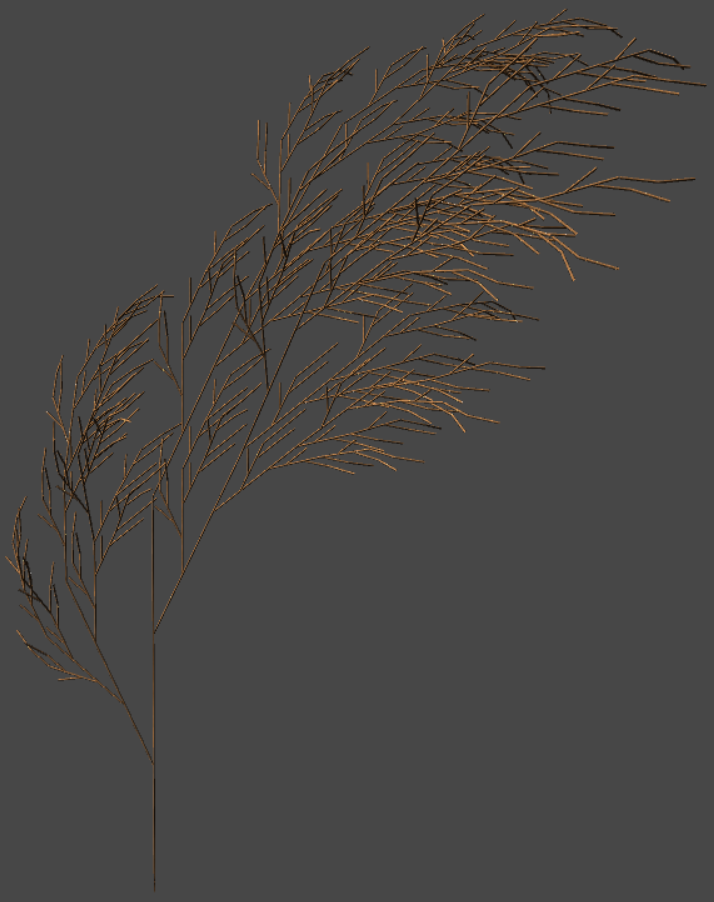
\includegraphics[width=0.8\linewidth]{siatka1}
\caption{Mesh without modification.\\Own source. \label{przyklad1.siatka}}
\end{subfigure}
%
\begin{subfigure}{.68\textwidth}
  \centering
  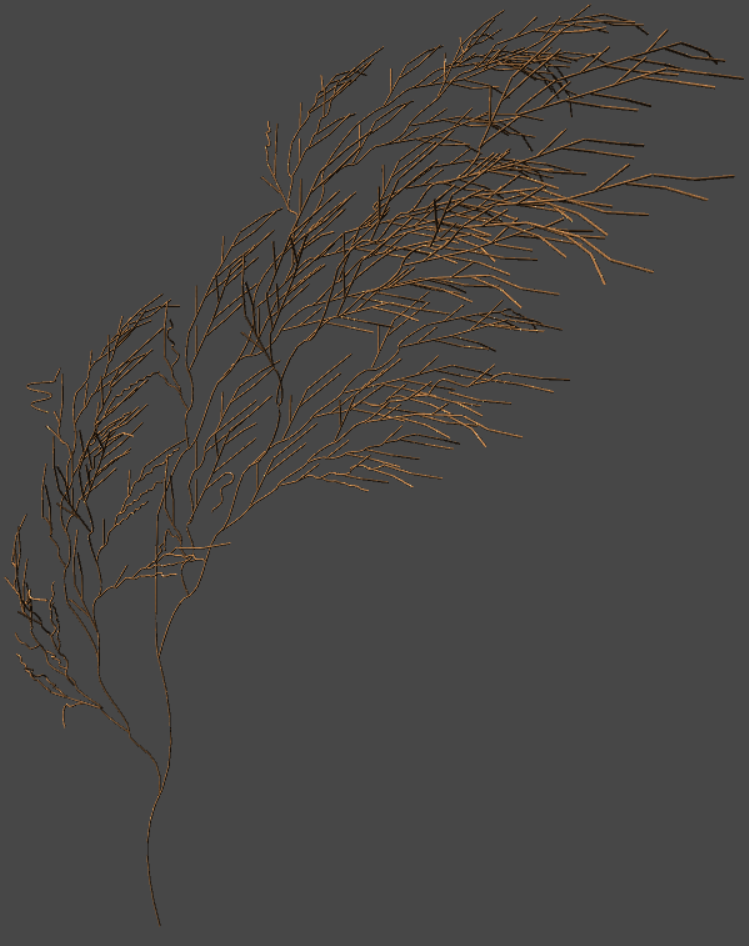
\includegraphics[width=0.8\linewidth]{siatkaMOD1}
\caption{Mesh after modification.\\Own source. \label{przyklad1.siatkaMOD}}
\end{subfigure}
\caption{Comparison of meshes for example  1.}
\label{przyklad1}
\end{figure}
%~~~~~~~~~~~~~~~~~~~~~~~~~~~~~~~~~~
\newpage

\subsection*{Example 2}
Next example have 171 branches, world forming tree have 24918 chars and 73700 vertices in model.\par
In this case the custom and longer rules have been used to make model looks like non-deterministic and more chaotic. Model before changes was shown at \figurename\ref{przyklad2.siatka}, and after changes at \figurename\ref{przyklad2.siatkaMOD}. In first example every variable had exactly one parameter without any mathematical operations, except $F(l \cdot 2)$. But in the second  every operation on parameter had to be evaluated and changed to float value, so the time of the calculation had increased significantly. Thanks to usage of multiple parameters and operation between them user can create more complicated structures, using less rules, but for the price of time for parameter evaluations.\\
Rules: \newline
\begin{equation*}
F(l)\rightarrow F(l\cdot2) 
\end{equation*}
\begin{equation*}
X(l,w) \rightarrow F(w\cdot l)[/(r\cdot l)X(l,w)-(r)X(w,w)]+(r)F(l)[\setminus(l)X(l,w)+(r)X(l,w)]-(r)F(w)
\end{equation*}
Axiom:
\begin{center}
X(1)
\end{center}
Number of iterations:
\begin{center}
5
\end{center}
Variables:
\begin{equation*}
r\rightarrow 17.2
\end{equation*}

\begin{figure}[!htp]
\centering
\begin{subfigure}{.68\textwidth}
  \centering
  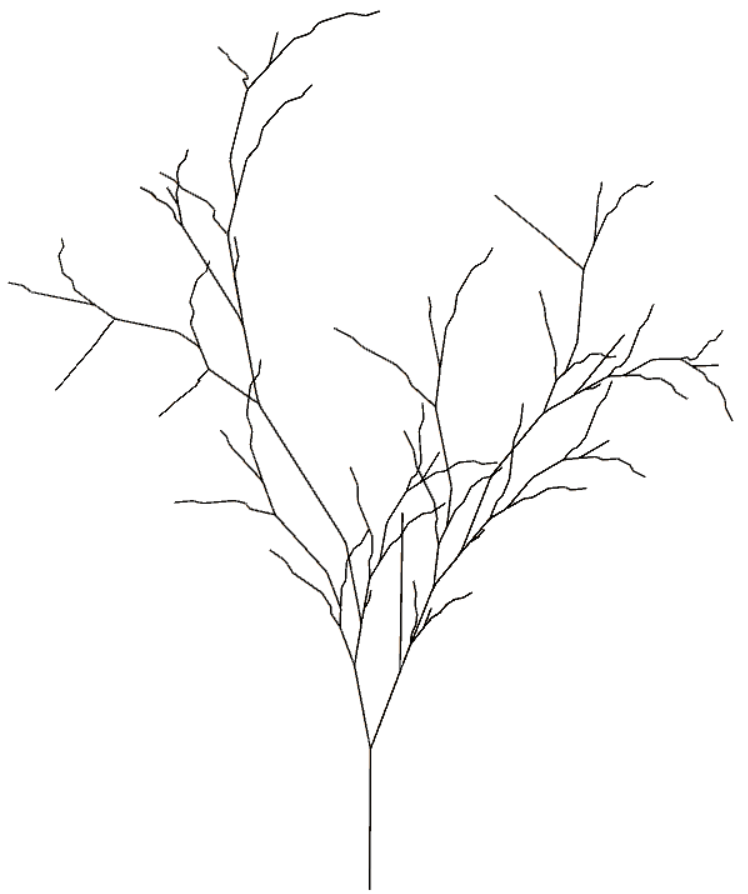
\includegraphics[width=0.8\linewidth]{przyklad2}
\caption{Mesh withouth modification.\\Own source. \label{przyklad2.siatka}}
\end{subfigure}
%
\begin{subfigure}{.68\textwidth}
  \centering
  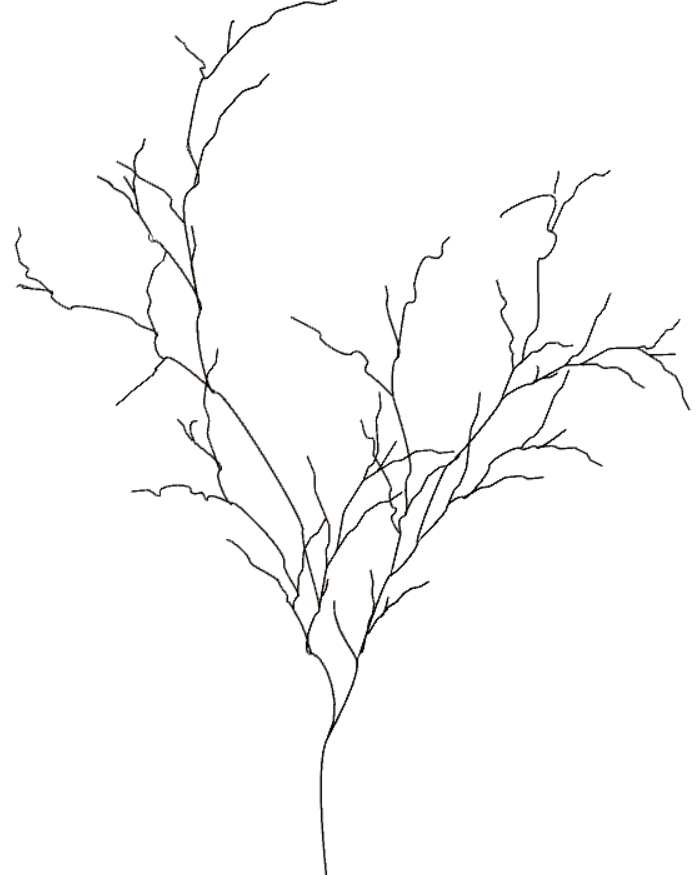
\includegraphics[width=0.8\linewidth]{przyklad2MOD}
\caption{Mesh after modification.\\Own source. \label{przyklad2.siatkaMOD}}
\end{subfigure}
\caption{Comparison of meshes for example  2.}
\label{przyklad2}
\end{figure}
\newpage

\subsection*{Example 3}
Last example have 214 branches, world world forming tree have 24918 chars and 73700 vertices in model. 
\figurename \ref{przyklad3.siatka} presents unchanged model of last example, \figurename \ref{przyklad3.siatkaMOD} same model after changes. Creating more complicated rule, based on those in example 2, and adding two more simple rules the model in example 3 is more non-deterministic and tree-like than other examples.
Rules: \newline
\begin{equation*}
F(l)\rightarrow F(l\cdot2) 
\end{equation*}
\begin{multline*}
X(l,w) \rightarrow F(w\cdot l)[/(r\cdot l)X(l,w)-(r)X(w,w)C(l)]\\
+(r)F(l)[G(l)\setminus(l)X(l,w)+(r)X(l,w)]-(r)F(w)-(r)F(w)
\end{multline*}
\begin{equation*}
G(l) \rightarrow F(l/5)[X(l,l)+(r\cdot k)]
\end{equation*}
\begin{equation*}
C(l) \rightarrow F(l/5)[X(l,l)/(r\cdot k)]
\end{equation*}
Axiom:
\begin{center}
X(1,2)
\end{center}
Number of iterations:
\begin{center}
5
\end{center}
Variables:
\begin{equation*}
r\rightarrow 23.5
\end{equation*}
\begin{equation*}
k\rightarrow 0.707
\end{equation*}





%~~~~~~~~~~~~~~~~~~~~~~~~~~~~~~~~~~
\begin{figure}[!htp]
\centering
\begin{subfigure}{.9\textwidth}
  \centering
  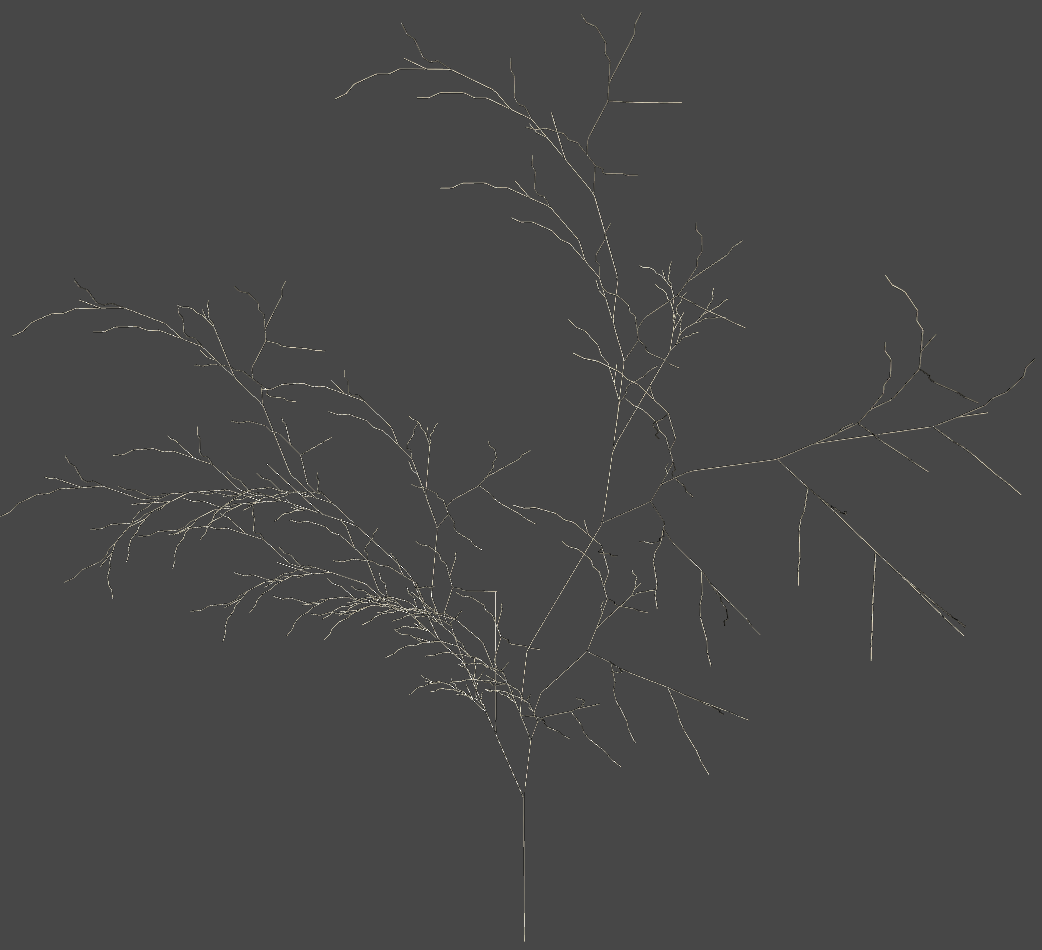
\includegraphics[width=0.8\linewidth]{przyklad3MOD}
\caption{Mesh without modification.\\Own source. \label{przyklad3.siatka}}
\end{subfigure}
%
\begin{subfigure}{.9\textwidth}
  \centering
  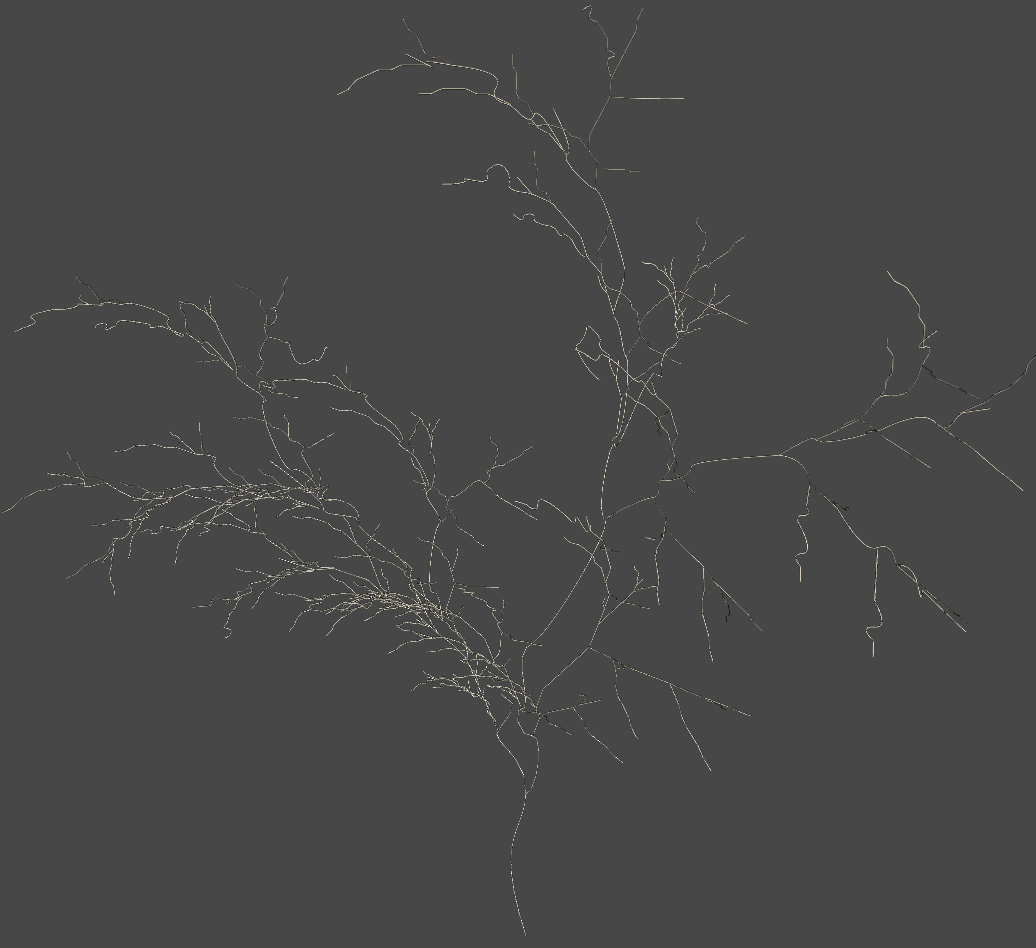
\includegraphics[width=0.8\linewidth]{przyklad3}
\caption{Mesh after modification.\\Own source. \label{przyklad3.siatkaMOD}}
\end{subfigure}
\caption{Comparison of meshes for example  3.}
\label{przyklad3}
\end{figure}
\newpage





\section{Conclusion}
By using technique described before the user can simply generate tree-like model in short time, small amount of vertices, and with ability to change every point of model using Bezier handles. Creating model with 300 branches using normal 3d  software would be very time consuming.We can move our work to machine and automatize process of modelling, using simple parametrized mathematical equations, without even knowing how the modelling software works. And we can do this inside game engine, without other programs.

To evaluate all string into float values the simple parser have been created.
Parser created with this implementation is simple, but creating possibility to evaluate more than 3 parameters, and operations between them, using approaches from this implementation would be very difficult. To ensure that every parameter would be evaluated properly whole implementation will be rewritten into new \textit{Boost Spirit X3} C++ library, and created as \textit{Dynamic-Link Library}. Unity,Unreal Engine and others game engines have ability to write plugins based on \textit{DLL} written in \textbf{C++}, so every engine could have their own implementation of this algorithm.
% use section* for acknowledgement



\begin{thebibliography}{99}
\bibitem{Herbaceus}Development models of herbaceous plants for computer imagery purposes,\url{http://dl.acm.org/citation.cfm?id=378503&CFID=841465770&CFTOKEN=79563252}
\bibitem{Sim} Simulation and visualization of fire using extended lindenmayer systems
\bibitem{WebTree}
L-system based interactive and lightweight web3D tree modeling
\bibitem{EnviroTree} Simulating tree growth based on internal and environmental factors
\bibitem{Spray}Simulating and visualising spray deposition on plant canopies
\bibitem{MLSystem}Musical L-Systems
\bibitem{LBrain}Evolved neurogenesis and synaptogenesis for robotic control: the L-brain model
\bibitem{L-Studio}L-studio, \url{http://algorithmicbotany.org/virtual_laboratory/}
\bibitem{ABartniak}Anna Bartniak
\bibitem{SelfSimi}How long is the coast of Britain?Statistical self-similarity and fractional dimension 
\bibitem{LHoud}\url{https://www.sidefx.com/docs/houdini/nodes/sop/lsystem}
\bibitem{prusinABOP}
Prusinkiewicz P., Lindermayer A. (2004) The Algorithmic Beauty of Plants.  wersja elektroniczna.
\bibitem{BSpline}
\url{http://mathworld.wolfram.com/B-Spline.html}
\bibitem{wlosy}
Fuhrer M. Hairs, Textures, and Shades: Improving the Realism of Plant Models Generated with L-systems. M.Sc. thesis, University of Calgary, August 2005. wersja elektroniczna
\bibitem{sca}
Runions A., Lane B., Prusinkiewicz P. Modeling Trees with a Space Colonization Algorithm,Department of Computer Science, University of Calgary, Canada ,Eurographics Workshop on Natural Phenomena (2007).
\bibitem{Sub} MacMurchy P., The Use of Subdivision Surfaces in the Modeling of Plants, THE UNIVERSITY OF CALGARY, April, 2004
\bibitem{VertexVertex} Smith C., On Vertex-Vertex Systems and Their Use in Geometric and Biological Modelling, THE UNIVERSITY OF CALGARY, April, 2006
\bibitem{houdiniZrodlo}
http://www.digitaltutors.com/tutorial/570-Procedural-Tree-Growth-Using-L-systems-in-Houdini
\bibitem{speedTreeZrodlo}
\url{http://www.speedtree.com/images/modeler_lrg.jpg}
\bibitem{unity}\url{https://unity3d.com/5}
\bibitem{splajn}\url{http://www.zobaczycmatematyke.krk.pl/025-Zolkos-Krakow/b-spline.html}
\bibitem {LMat} Rozenberg G., Salomaa A. \textit{The mathematical theory of L systems}, Academic Press, New York, 1980

\end{thebibliography}

\ifdefined\PROCINCLUDED
%
\else
\end{document}
\fi
